\documentclass[
	% -- opções da classe memoir --
	12pt,				% tamanho da fonte
	openright,			% capítulos começam em pág ímpar (insere página vazia caso preciso)
	twoside,			% para impressão em verso e anverso. Oposto a oneside
	a4paper,			% tamanho do papel. 
	% -- opções da classe abntex2 --
	%chapter=TITLE,		% títulos de capítulos convertidos em letras maiúsculas
	%section=TITLE,		% títulos de seções convertidos em letras maiúsculas
	%subsection=TITLE,	% títulos de subseções convertidos em letras maiúsculas
	%subsubsection=TITLE,% títulos de subsubseções convertidos em letras maiúsculas
	% -- opções do pacote babel --
	english,			% idioma adicional para hifenização			
	brazil				% o último idioma é o principal do documento
	]{abntex2}

% ---
% Pacotes básicos 
% ---
\usepackage{lmodern}
\usepackage{lastpage}			% Usado pela Ficha catalográfica
\usepackage{indentfirst}		% Indenta o primeiro parágrafo de cada seção.
\usepackage[utf8]{inputenc}
\usepackage[T1]{fontenc}
\usepackage[brazilian,hyperpageref]{backref}	 % Paginas com as citações na bibl
\usepackage[alf]{abntex2cite}	% Citações padrão ABNT
\usepackage{microtype} 			% para melhorias de justificação

% \usepackage[fixlanguage]{babelbib}
\usepackage{amsmath}
\usepackage[colorinlistoftodos]{todonotes}
\usepackage{tabularx}
\usepackage{multirow}
\usepackage{graphicx}
\usepackage{listings}
\usepackage{url}
\usepackage{float}
\usepackage{comment}
\usepackage{caption}
\usepackage{color}
%\usepackage{nomencl}
%\usepackage{fontspec}
%\usepackage{titlesec}
\definecolor{lightgray}{rgb}{0.95,0.95,0.95}
\linespread{1.25}

% --- 
% CONFIGURAÇÕES DE PACOTES
% --- 

% ---
% Configurações do pacote backref
% Usado sem a opção hyperpageref de backref
%\renewcommand{\backrefpagesname}{Citado na(s) página(s):~}
% Texto padrão antes do número das páginas
%\renewcommand{\backref}{}
% Define os textos da citação
%\renewcommand*{\backrefalt}[4]{
%	\ifcase \#1 %
%		Nenhuma citação no texto.%
%	\or
%		Citado na página \#2.%
%	\else
%		Citado \#1 vezes nas páginas \#2.%
%	\fi}%
% ---

% ---
% Informações de dados para CAPA e FOLHA DE ROSTO
% ---
\titulo{Sistema de Monitoramento Residencial de Uso de Energia}
\autor{Henrique Sussumu Matsui Kano \& Mi Che Li Lee}
\local{São Paulo}
\date{2015}
\orientador{Professor Doutor Carlos Eduardo Cugnasca}
\instituicao{%
  Escola Politécnica da Universidade de São Paulo
  \par
  Departamento de Computação e Sistemas Digitais
  \par
  Graduação}
\tipotrabalho{Dissertação (Graduação)}
% O preambulo deve conter o tipo do trabalho, o objetivo, 
% o nome da instituição e a área de concentração 
\preambulo{Dissertação apresentada à Escola Politécnica da Universidade de São Paulo para a conclusão do curso de graduação em Engenharia de Computação}
% ---

% ---
% Configurações de aparência do PDF final

% alterando o aspecto da cor azul
\definecolor{blue}{RGB}{41,5,195}

% informações do PDF
\makeatletter
\hypersetup{
     	%pagebackref=true,
		pdftitle={\@title}, 
		pdfauthor={\@author},
    	pdfsubject={\imprimirpreambulo},
	    pdfcreator={LaTeX with abnTeX2},
		pdfkeywords={abnt}{latex}{abntex}{abntex2}{trabalho acadêmico}, 
		colorlinks=true,       		% false: boxed links; true: colored links
    	linkcolor=blue,          	% color of internal links
    	citecolor=blue,        		% color of links to bibliography
    	filecolor=magenta,      		% color of file links
		urlcolor=blue,
		bookmarksdepth=4
}
\makeatother
% --- 

% --- 
% Espaçamentos entre linhas e parágrafos 
% --- 

% O tamanho do parágrafo é dado por:
\setlength{\parindent}{1.3cm}

% Controle do espaçamento entre um parágrafo e outro:
\setlength{\parskip}{0.2cm}  % tente também \onelineskip

% ---
% compila o indice
% ---
\makeindex
% ---


\lstset{%
  backgroundcolor=\color{lightgray},
  commentstyle=\color{gray},
  basicstyle=\footnotesize\ttfamily,
  breaklines=true, 
  tabsize=2,
  captionpos=b
}

\begin{document}
\begin{titlepage}

\begin{center}
\vspace{30mm}
\large
Escola Politécnica da Universidade de São Paulo\\
Henrique Sussumu Matsui Kano\\
Mi Che Li Lee

\vspace{90mm}
\Large
Sistema de Monitoramento Residencial de Uso de Energia

\vfill
São Paulo\\
2015

\end{center}

\end{titlepage}


\frontmatter
\addcontentsline{toc}{chapter}{Sumário}   
\tableofcontents

\cleardoublepage 
\addcontentsline{toc}{chapter}{Lista de Figuras}  
\listoffigures  

\cleardoublepage 
\addcontentsline{toc}{chapter}{Lista de Tabelas} 
\listoftables  

\mainmatter

\pagestyle{headings}

\chapter{Introdução}
\label{Cap:Introducao}

\section{Objetivo}
\label{Sec:objetivo}

O trabalho descreve a construção de um sistema para monitorar o uso de energia dentro da residência. O sistema consiste de dispositivos interligados por uma rede sem fio, composta por: uma rede local de sensores  que fará o sensoriamento dos parâmetros e se comunicará com uma aplicação em nuvem e a aplicação em nuvem, que apresentará as medidas enviadas pelos sensores numa interface simples e intuitiva, permitindo também o acesso remoto.

\section{Motivação}
\label{Sec:motivacao}

A primeira das principais motivações do grupo foi a preocupação do desenvolvimento de um sistema que englobasse diversas áreas vistas ao longo do curso de engenharia para que fosse possível, ao final do trabalho, uma reflexão pessoal dos integrantes quanto a evolução técnica desses tópicos. A segunda motivação é a resolução de um problema muito comum na atualidade, que é o encarecimento da energia,  utilizando como instrumentos as técnicas de automação residencial.

Tem-se como expectativa um produto aplicável no dia-a-dia e com alguns diferenciais em relação aos produtos existentes no mercado \cite{green_ant_site}, no sentido que usará equipamentos disponíveis no mercado com um resultado satisfatório. O trabalho descreve um sistema no qual pode-se identificar o consumo elétrico por equipamento, ao invés do consumo da rede residencial como um todo e, além disso, ser adaptável às metas de consumo, considerando a experiência do usuário.

\section{Justificativa}
\label{Sec:justificativa}

Em 2015, devido à escassez de chuvas, houve uma queda significativa no nível dos reservatórios das principais hidrelétricas do Brasil e o uso mais intenso de termelétricas. Isso provocou reajustes altos, encarecendo a energia do país e o custo foi repassado para os consumidores finais \cite{news_g1}  \cite{news_secretaria_de_energia}. Por isso é imprescindível a tomada de atitudes por parte da população tanto para controlar os gastos na conta de luz quanto para a redução do consumo de eletricidade nas suas residências,  aliviando a carga do sistema de produção e distribuição de eletricidade.

Trazendo o problema para a área da engenharia, e sabendo da grande gama de tecnologia disponível, a criação de ferramentas que podem nos auxiliar na monitoração e controle de gastos de energia é favorecida. Existem sistemas no mercado, ou prestes a entrar no mercado, que realizam a função de monitorar o consumo de energia residencialmente como a OpenEnergyMonitor\cite{open_energy_monitor}, Neurio\cite{neurio_site}, Green Ant\cite{green_ant_site}. Entretanto há a preocupação de se desenvolver um sistema, em alguns meses, aproveitando a onda de desenvolvimento e hardware/software open-source, com padronizações e a comercialização de tecnologias de redes de sensores sem fio. Um sistema pode ser assim construído modularmente, permitindo o desenvolvimento rápido de protótipos altamente personalizáveis, de pouco custo e que consomem pouca bateria.

O sistema permite medir o consumo por aparelho, ao invés do consumo da rede elétrica residencial como um todo, sendo possível, então detectar possíveis aparelhos “vilões”, por excesso de consumo de energia.

O sistema dá uma visão quantitativa ao usuário, e isso é fundamental para a tomada de decisões conscientes, resultando em uma administração eficiente dos gastos residenciais.

\section{Organização}
\label{Sec:organizacao}

O documento segue o seguinte formato: no capítulo dois são apresentados os conceitos do projeto e diagramas do sistema de uma forma genérica, sem mencionar nomes ou marcas de componentes, porém são mencionados os principais módulos do sistema, assim como os nomes utilizados para esses módulos no trabalho todo.

No capítulo três são exploradas as peças do sistemas assim como as funcionalidades dele.

No capítulo quatro é apresentado o método de projeto adotado pelo grupo durante o desenvolvimento do projeto, da parte de projeto até sua implementação e conclusão.

No capítulo cinco é detalhado mais sobre como foi feita a implementação, como os passos feitos na construção dos módulos do sistema, citando detalhes mais técnicos de problemas, soluções e mudanças de projeto em relação ao procedimento teórico criado.

No capítulo seis é detalhado o procedimento de aceitação do sistema através da aplicação de um plano de testes e seus resultados.

No capítulo sete são apontadas algumas considerações finais como comentários e resultados atingidos.

Além do capítulo oito são citadas algumas idéias que poderiam ser aplicadas a trabalhos futuros.
\chapter{Aspectos Conceituais}
\label{Cap:conceitos}

As técnicas de monitoramento e sensoriamento podem ser usados para as mais diversas funções e implementadas de diversas maneiras. Nesse trabalho, são usadas técnicas, arquiteturas e tecnologias para monitorar o consumo de energia elétrica em um ambiente residencial por uma rede de sensores na qual cada sensor da rede transmite seus dados a um componente central que se comunica com uma aplicação em nuvem  \cite{low_cost_wireless_sensor_network_SMF_master_thesis}.

São abordados vários conceitos vistos em aula. Um deles engloba o universo dos protocolos e componentes de uma rede sem fio. Isso envolve o estudo do protocolo que será utilizado nesse projeto, que é o ZigBee, devido ao seu grande uso na área o que implica em uma grande fonte de informações sobre este\cite{xbee_book}\cite{sensor_network_book}\cite{low_cost_wireless_sensor_network_SMF_master_thesis}. Junto a isso são estudados a montagem de circuitos de sensores associados a microcontroladores e a captação dos dados dos sensores por uma central.

Além disso é estudado o desenvolvimento de aplicações para Web e arquitetura de sistemas.

%\section{Circuito AC}
%\label{Sec:ac}

%\todo[inline, color=red!40]{Fazer}


\section{Arquitetura MVC }
\label{Sec:MVC}

A arquitetura MVC é a mais utilizada nos dias atuais para a concepção de aplicativos web, uma vez que ela permite a implementação de um sistema de melhor manutenção ao separar responsabilidades nas camadas de Model, View e Controller \cite{MVC_design} (figura \ref{fig:mvc})

\begin{figure}
\centering
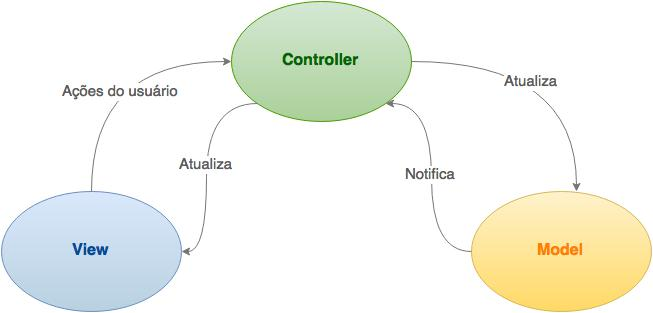
\includegraphics[width=10cm,keepaspectratio]{figuras/MVC.jpg}
\caption{\label{fig:mvc} Arquitetura MVC}
\end{figure}

\textbf{Model:} A camada Model representa a primeira camada de interação com qualquer banco de dados que possa estar sendo usado na aplicação. Ela é responsável por obter, processar, validar dados do banco de dados.

\textbf{View:} A view é responsável por usar as informações disponibilizadas para produzir qualquer interface de apresentação que a aplicação pode necessitar.

\textbf{Controller:} essa camada lida com as requisições dos usuários. É responsável por se comunicar com a camada Model para realizar operações de busca ou armazenamento de dados e repassar os dados obtidos para a camada View, que irá gerar uma saída resultante para o usuário.

MVC é um padrão de projeto de software recomendado para aplicações de desenvolvimento rápido, de fácil manutenção e modular. E foi escolhido como o ideal para um projeto com um tempo limitado de desenvolvimento e possibilita a divisão fácil de tarefas entre os membros da equipe

\section{Wireless Sensor Network }
\label{Sec:WSN}
Wireless Sensor Network, também conhecido como WSN, é um termo genérico que descreve sistemas que tem como objetivo o sensoriamento e monitoração de algum objeto em uma certa área, em pelo menos uma variável (temperatura, umidade, pressão, cor, etc). Os desafios de tais estruturas se resumem a \cite{WSN_survey_JYBMDG_article}: sensores e nós que compõem a rede e podem ter a função de sensoriamento ou de retransmitir dados a um outro nó ou à estação base para serem salvos e devem formar sozinhos uma rede que consiga garantir que os dados sensoriados chegem à base, protocolo de comunicação entre nós, que podem afetar significantemente no consumo de energia, atrasos de comunicação e eficiência do sistema como um todo, fontes de energia dos nós limitada e soluções de coleta de energia. 

\section{Padrão ZigBee e o XBee}
\label{Sec:ZigBee_XBee}
 Para realizar a comunicação sem fio entre os módulos coordenador e sensor, foi necessária a escolha de um padrão para fazer esse intermédio de mensagens. Para realizar tal escolha foram levados em consideração principalmente a eficiência energética que o padrão tem, confiabilidade e escalabilidade. Apesar de existirem opções melhores em certos aspectos, como o Bluetooth Low Energy na área de consumo de energia \cite{BLE_MHABAL}, o ZigBee possui um certo balanceamento das características procuradas, sendo uma solução mais genérica \cite{CG_JP_survey}. Com a existência do XBee, um dispositivo que implementa o ZigBee, é mais interessante adotar tal padrão, uma vez que esse dispositivo facilita a produção do protótipo final.

 O padrão ZigBee e o dispositivo XBee possuem muitas características configuráveis e que podem servir a várias aplicações\cite{xbee_book}, porém duas delas são de maior interesse para o trabalho: o baixo consumo de energia e os modos de operação. O XBee pode ser configurado para operar em um dos dois modos: AT ou API. No modo AT há apenas o envio de dados ponto-a-ponto na rede, porém, no modo API, é possível agir na rede durante sua operação com mudanças de configuração de nós, broadcast, confirmação de entrega de pacotes e identificação do endereço dos dados recebidos, o que dá ao sistema um maior controle do todo \cite{xbee_documentation}
 
\section{Topologias de Rede}
\label{Sec:Redes_topologias}
 Como os nós dos sensores formam uma rede, é necessário analisar as possibilidades de redes.  Como são usados XBees para formar essa rede de sensores, deve-se atentar aos tipos de rede possíveis \cite{xbee_book} \cite{xbee_documentation}.
 
\begin{figure}[H]
\centering
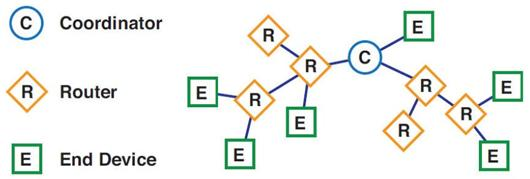
\includegraphics[width=10cm,keepaspectratio]{figuras/zigbee_network_topology.jpg}
\caption{\label{fig:zigbee_network} Topologia de uma rede zigbee}
fonte: \url{http://ftp1.digi.com/support/documentation/html/90001399/90001399_A/Files/XBee-concepts.html}
\end{figure}
 
 A rede ZigBee é composta por nós que podem ser de três tipos:
 \begin{itemize}
\item{Coordenador}: Nó destino (final) de todos os outros nós, concentrando os dados de todos os nós. Todas as redes possuem apenas um nó desse tipo e como esse tipo de nó não possui a capacidade de dormir ele não deveria ficar em um dispositivo com uma bateria limitada.
\item{Roteador}: Funciona apenas como uma ponte intermediária entre os endpoints e o coordenador, podendo se comunicar com todos os outros tipos de nós, mas também não possuem a capacidade de dormir, logo não podem ser energizados com uma bateria limitada. Normalmente são usados para estender a área de uma rede, aumentando o alcance sensoreada da rede como um todo.
\item{Dispositivos finais}: Nós que são as pontas da rede e que normalmente estão ligados aos sensores. Esses tem a capacidade de dormir e conservar energia enquanto não transmitem e só não conseguem se comunicar com outros nós do mesmo tipo diretamente;

Dadas essas especificações e limitações, as redes formadas por esses componentes podem ser de de três tipos \cite{xbee_book}: estrela, árvore ou mesh. Na estrela os dispositivos finais conversam diretamente com o coordenador, na rede mesh os dispositivos finais estão intermediados por uma malha de roteadores que se organizam para encontrar o melhor caminho de roteadores de um dispositivo final até o coordenador e a árvore é um subcaso da rede mesh onde, devido a bloqueios físicos ou distâncias entre os roteadores, a rede acaba por se tornar uma árvore ou um grafo onde o caminho de um dispositivo final até o coordenador praticamente não possui alternativas.

\end{itemize}


\mychapter{Especificação do Projeto}
\label{Cap:especificacao}
\paragraph{
	O sistema será composto por duas partes: hardware, ou seja, os componentes como roteadores, processadores, sensores, entre outros; e software, identificado como o aplicativo de interface entre o usuário e os dados coletados.
}
\paragraph{
	O sistema está brevemente descrito através da Figura 1 e a disposição dos componentes através do diagrama de implantação da figura 2:
}
\begin{figure}
\centering
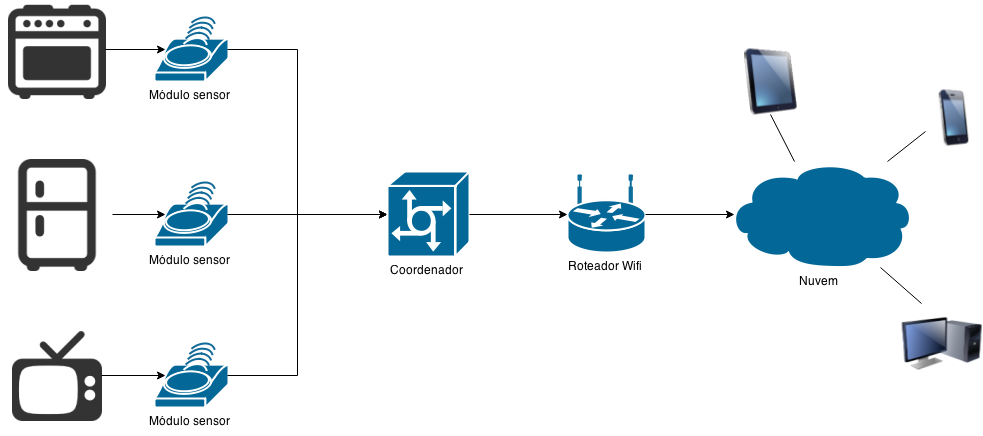
\includegraphics[width=1\textwidth]{figuras/esqueminha.png}
\caption{\label{fig:esqueminha} Esquema do Projeto}
\end{figure}

\begin{figure}
\centering
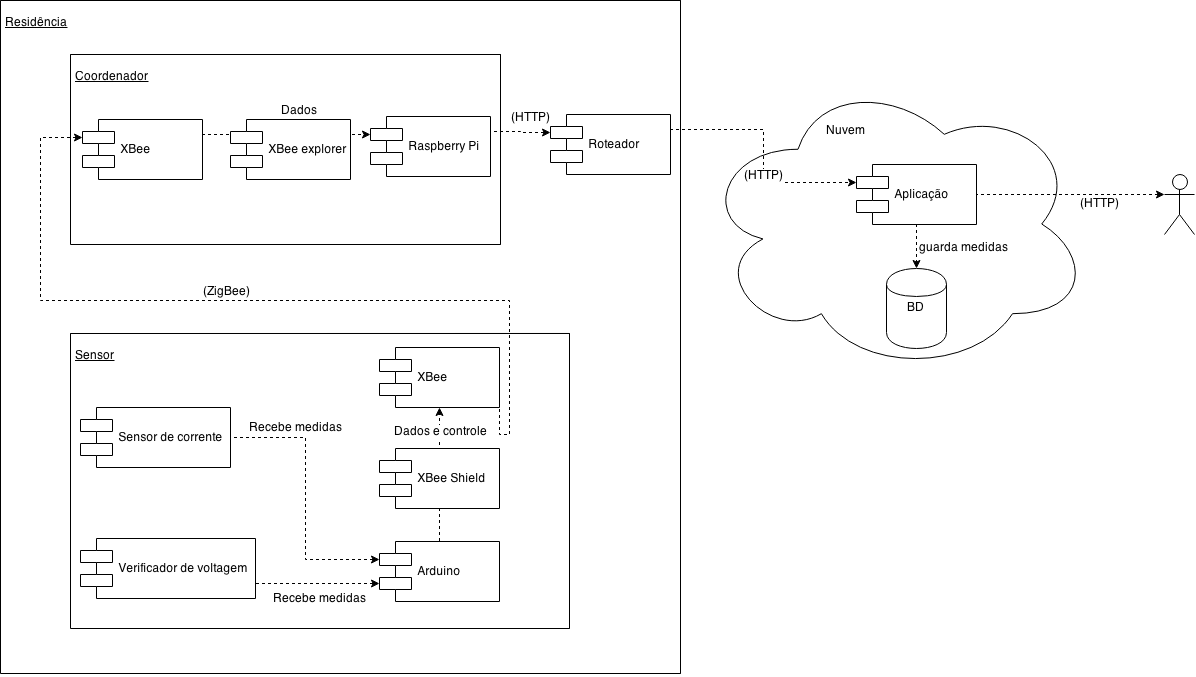
\includegraphics[width=1\textwidth]{figuras/diagrama_implantacao.png}
\caption{\label{fig:diagrama_implantacao} Diagrama de implantação}
\end{figure}
\paragraph{
	A parte de hardware está separado em dois módulos principais: o módulo de sensoriamento e um módulo coordenador e a parte de software se resume à parte da aplicação web na nuvem.
}
\section{Hardware}
\label{Sec:hardware}
\subsection{Módulo sensor}
\paragraph{
	O módulo sensor vai ser responsável por medir e transmitir as informações necessárias para calcular o consumo de energia do equipamento acoplado.
}
\paragraph{
	Os componentes físicos do módulo sensor são:
}
\begin{itemize}
\item Circuito Verificador de Voltagem
\item Sensor de Corrente (Non-invasive AC Current Sensor)
\item Arduino Uno - R3
\item XBee Shield
\item XBee 2mW PCB Antenna - Series 2
\end{itemize}

\subsection{Coordenador}
\paragraph{
	O módulo coordenador vai ser responsável por fazer requisições para os módulos sensores, tratar os dados de consumo e enviar ao aplicativo.
}
\paragraph{
	Os componentes do coordenador são:
}
\begin{itemize}
\item Kit Raspberry Pi2 + Fonte + Microsd 8gb + Wifi Usb
\item XBee Explorer Dongle
\item XBee 2mW PCB Antenna - Series 2
\end{itemize}

\subsection{Circuitos}
\subsubsection{Verificador de Tensão}
\paragraph{
No circuito de cada módulo de sensor, são feitas detecções da voltagem (110V ou 220V) para cálculos de potência. O circuito da Figura 3.3 foi simulado no PSpice para esse propósito, com componentes com parâmetros não finais, para uma análise lógica do bloco. O objetivo do circuito da figura dois é indicar se a tensão na tomada é 220V ou 110V, retornando 5V ou 0V, respectivamente.
}
\begin{figure}[H]
\centering
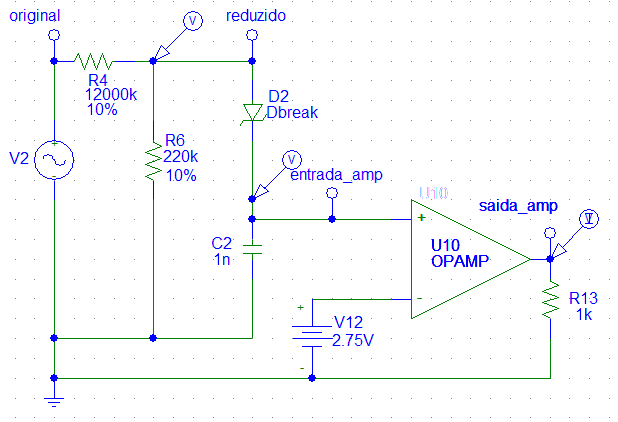
\includegraphics[width=1\textwidth]{figuras/voltage-circuit.png}
\caption{\label{fig:voltage-circuit} Diagrama de blocos do circuito que verifica a tensão}
\end{figure}

\subsection{Peças}
\subsubsection{Non-invasive AC current sensor}
\subsubsection{Raspberry Pi 2 modelo B}
\begin{figure}[H]
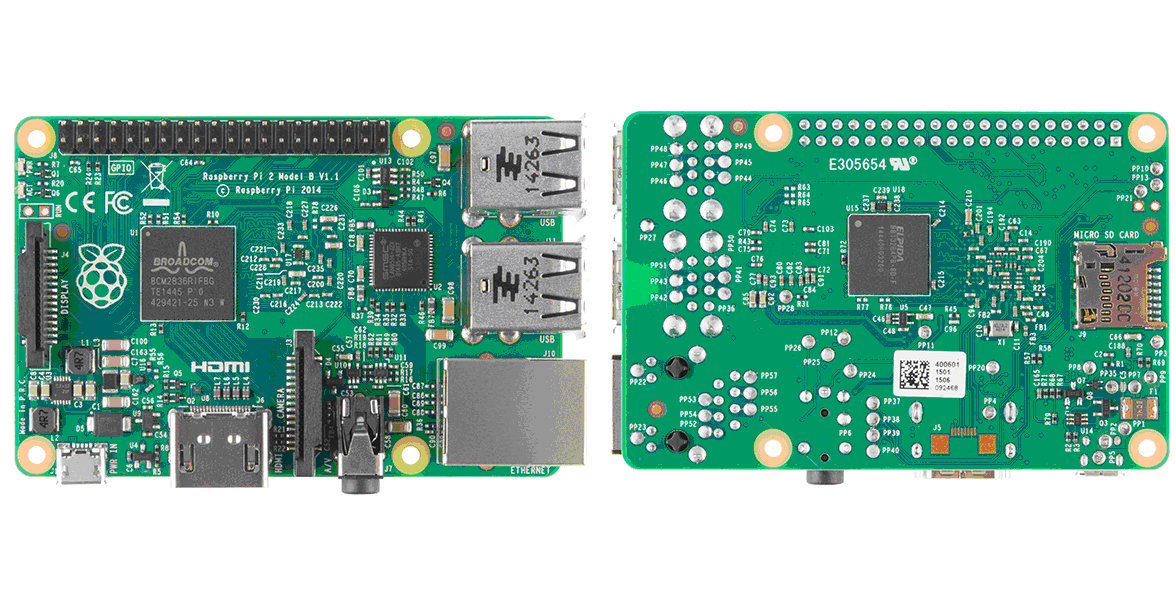
\includegraphics[width=1\textwidth]{figuras/raspberry_pi.png}
\caption{\label{fig:raspberry pi} Raspberry pi 2 modelo B}
\end{figure}
\paragraph{
A Raspberry Pi 2 Modelo B (figura 3.4) é o computador utilizado no sistema para receber os dados enviados pelos módulos sensores, tratá-los e enviar para o aplicativo. Foi escolhido o Raspberry Pi 2 - Model B por ser mais veloz, por possuir mais entradas USB e ser de alta disponibilidade no mercado, por um preço razoável. O kit inclui a fonte, um cartão microSD de 8GB e um adaptador Wifi USB.
}
\begin{itemize}
\item{A 900MHz quad-core ARM Cortex-A7 CPU}
\item{1GB RAM}
\item{40 pinos GPIO}
\item{saída Full HDMI}
\item{porta Ethernet}
\item{entrada para cartão Micro SD}
\item{4 entradas USB}
\end{itemize}

\subsubsection{Arduino UNO}
\begin{figure}[H]
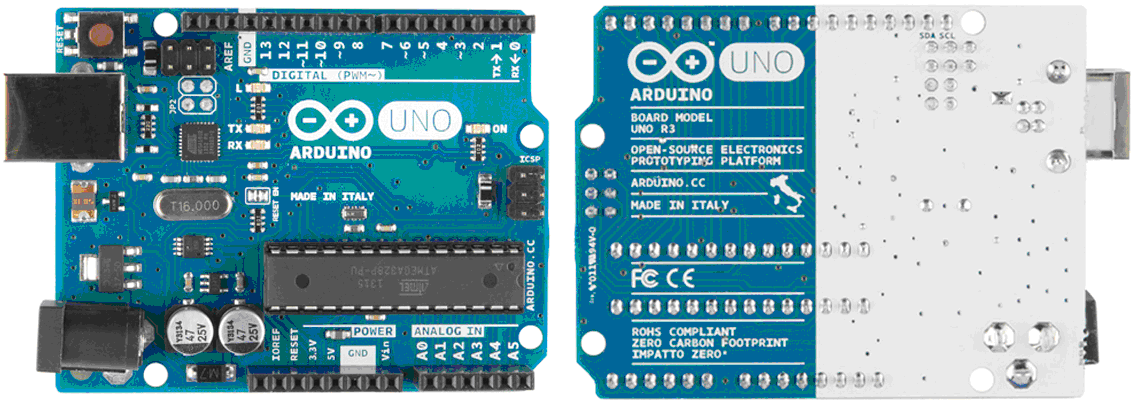
\includegraphics[width=1\textwidth]{figuras/arduino_uno.png}
\caption{\label{fig:arduino uno} Arduino UNO}
\end{figure}
\paragraph{
Arduino é uma placa programável open-source . No projeto em questão é utilizado como o microcontrolador, que receberá os dados do sensor, fará um tratamento e terá o envio programado desses para o coordenador. Pelo Arduino ser programável e possuir uma interface muito amigável, simplifica essa ponte entre a coleta de dados e a transmissão.
}
\begin{itemize}
\item{microcontrolador ATmega328}
\item{Voltagem de entrada - 7-12V}
\item{14 Pinos Digital I/O (6 PWM de saída)}
\item{6 Inputs Analógicos}
\item{32k de memória Flash}
\item{16Mhz de Relógio}
\end{itemize}

\subsubsection{XBee}
\begin{figure}[H]
\begin{center}
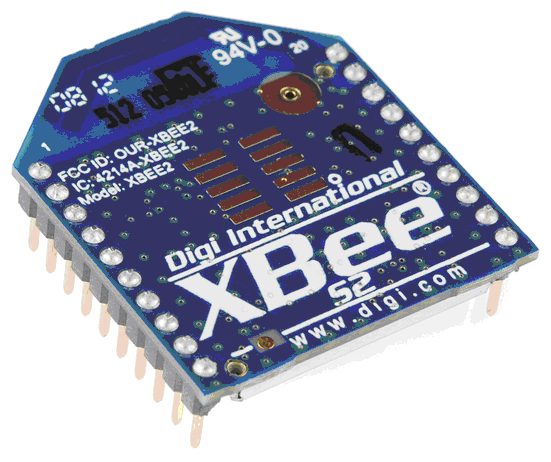
\includegraphics[width=5cm,height=5cm,keepaspectratio]{figuras/xbee_serie2.png}
\caption{\label{fig:xbee} XBee serie 2}
\end{center}
\end{figure}
\paragraph{
É um módulo que permite uma comunicação simples e confiável entre microcontroladores, computadores, sistemas através de uma porta serial. Pode ser utilizado em redes ponto-a-ponto e multi-ponto. Foram escolhidos módulos da série 2 pois são configuráveis.
Algumas outras especificações são:
}
\begin{itemize}
\item{entradas de 3.3V @ 40mA}
\item{transmissão de dados máxima de 250kbps}
\item{potência de saída: 2mW (+3dBm)}
\item{alcance mãximo de 120m}
\item{08 pinos digitais entrada/saída}
\item{encriptação 128-bit}
\item{configuração local ou remota}
\item{conector de antena RPSMA}
\end{itemize}

\subsubsection{XBee Explorer Dongle}
\begin{figure}[H]
\begin{center}
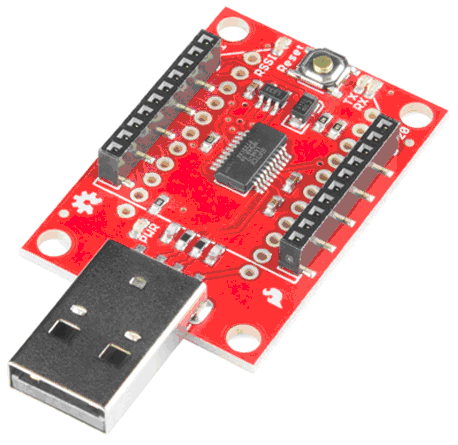
\includegraphics[width=5cm,height=5cm,keepaspectratio]{figuras/xbee_explorer_dongle.png}
\caption{\label{fig:xbee explorer dongle} XBee Explorer Dongle}
\end{center}
\end{figure}
\paragraph{
É um módulo com porta USB que faz a conexão do módulo XBee a um computador. Isso é necessário para ter acesso aos pinos de comunicação serial e de programação. Ele possui um conversor USB-serial, que traduz os dados entre o computador e o XBee. Possui um botão de reset e um regulador de voltagem para suprir a voltagem necessária para XBee. Além disso possui 4 leds para debug: RX, TX, RSSI e indicador de energia. No projeto, este módulo é utilizado para fazer as configurações iniciais de todos os XBees e para conectar o XBee coordenador ao Raspberry Pi.
}

\subsubsection{XBee Shield}
\begin{figure}[H]
\begin{center}
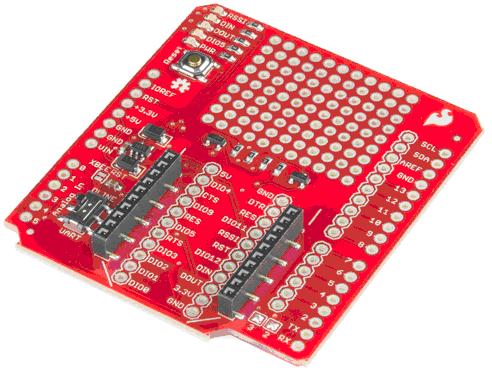
\includegraphics[width=5cm,height=5cm,keepaspectratio]{figuras/xbee_shield.png}
\caption{\label{fig:xbee shield} XBee shield do arduino UNO}
\end{center}
\end{figure}
\paragraph{
É um módulo que faz a conexão entre um módulo XBee e um Arduino. Ele possui opções para escolher se a conexão vai ser nos pinos UART ou qualquer outros pinos digitais do Arduino. A alimentação de 5V vinda do Arduino é regulada para 3.3V VDC antes de chegar no módulo XBee. O XBee Shield inclui LEDs para indicar a utilização dos pinos DIN, DOUT, RSSI e DIO5 do XBee. É usado um módulo XBee Shield para cada par XBee + Arduino.
}

\subsubsection{Arduino Stackable Header Kit - R3}
\begin{figure}[H]
\begin{center}
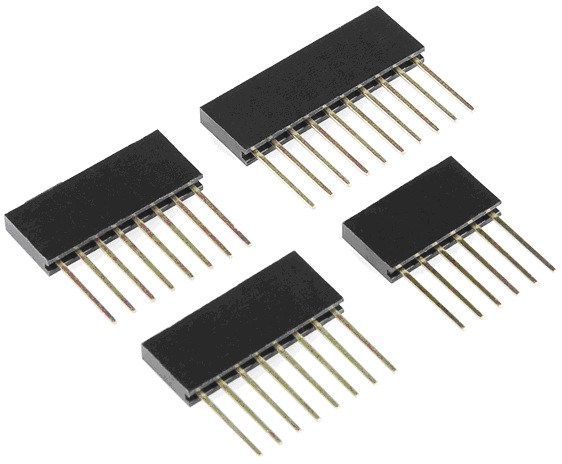
\includegraphics[width=5cm,height=5cm,keepaspectratio]{figuras/headers.png}
\caption{\label{fig:xbee shield headers} Headers usados no XBee shield}
\end{center}
\end{figure}
\paragraph{
São conectores usados para encaixar o módulo XBee Shield no Arduino Uno R3. Estão inclusos 4 headers, 2 x 8 pinos, 1 x 10 pinos e 1 x 6 pinos, suficientes para 1 módulo XBee Shield. Como há 2 sensores no projeto, serão usados 2 kits, com um adicional de reserva.
}

\section{Software}
\label{Sec:software}
\paragraph{
Coletado os dados, resta mostrar informações úteis ao usuário. Com o consumo de corrente e a voltagem da tomada, é possível calcular a potência e alguns outros dados interessantes para o usuário. O aplicativo desenvolvido nesse trabalho será responsável por esse tratamento e a visualização dos dados coletados pelos sensores. As funções principais são as seguintes:
}
\begin{itemize}
\item{realizar login}
\item{criar planos de consumo mensal máximo}
\item{visualizar o consumo através de gráficos por equipamento ou total}
\item{calcular o custo do consumo dos equipamentos por período}
\item{exportar os dados de consumo de um equipamento (ou mais)}
\item{importar os dados de consumo de um equipamento (ou mais)}
\end{itemize}
\subsection{Classes e atributos}
\textbf{Classe}: Equipment\\
\textbf{Descrição}: um equipamento monitorado\\	
\textbf{Atributos:}
\begin{enumerate}
  \item id (integer): Identificador do equipamento
  \item name (String): Nome do equipamento
  \item description (Text): descrição do equipamento 
  \item nominal\_power (float): potência do equipamento descrita no manual do equipamento 
  \item measurement\_unit (String): unidade do valor dado em nominal\_power
  \item approximated\_consumption (float): consumo aproximado do equipamento dado pelo fabricante 
\end{enumerate}

\textbf{Classe}: Sensor\\
\textbf{Descrição}: um sensor do sistema\\	
\textbf{Atributos:}
\begin{enumerate}
	\item id (integer): identificador do sensor dentro do software.
	\item name (String): nome dado pelo usuário para o sensor
	\item code (String): identificador do sensor entre outros sensores. Informação configurada no próprio módulo do sensor.
	\item equipment\_id (integer): equipamento a qual está associado
\end{enumerate}

\textbf{Classe}: Consumption\\
\textbf{Descrição}: Representa uma medida feita de um equipamento em um dado instante\\	
\textbf{Atributos:}
\begin{enumerate}
	\item id (integer): identificador do consumo
	\item moment (DateTime): a data e a hora de quando foi feita a medida
	\item current (float): corrente no momento da medida em amperes
	\item voltage (float): voltagem do tomada do equipamento. 220V ou 110V
\end{enumerate}

\subsection{Classes e atributos}
	\textbf{Classe}: User\\
	\textbf{Descrição}: Representa um usuário do sistema\\	
	\textbf{Atributos:}
\begin{enumerate}
	\item id (integer): identificador do usuário
	\item name (String):  Nome do usuário
	\item username (String): Nome de usuário usado para efetuar o login
	\item password (String com Criptografia): Senha do usuário usada para efetuar o login
    \item income\_type (String): O tipo de renda do usuário, Residencial ou Residencial de baixa renda, definida pela AES eletropaulo.
\end{enumerate}

\subsection{Classes e atributos}
	\textbf{Classe}: Goal\\
	\textbf{Descrição}: Representa uma meta de consumo por mês.\\
	\textbf{Atributos:}
\begin{enumerate}
	\item id (integer): identificador da meta
	\item name (String):  Nome da meta
	\item value\_in\_percent (float): Consumo pretendido em percentagem (em relação ao mês anterior)
	\item yearmonth\_start (DateTime): Mês/Ano de início do período da meta
    \item yearmonth\_end (DateTime): Mês/Ano de fim do período da meta
\end{enumerate}

\subsection{Classes e atributos}
	\textbf{Classe}: AESRate\\
	\textbf{Descrição}: Representa a taxa de conversão da AES eletropaulo de kilowatts hora para reais. Esses valores são obtidos através do site da AES Eletropaulo: \url{https://www.aeseletropaulo.com.br/poder-publico/prazos-e-tarifas/conteudo/tarifa-de-energia-eletrica}\\
	\textbf{Atributos:}
\begin{enumerate}
	\item id (integer): identificador da taxa de conversão
	\item value (float): O valor da taxa de conversão no instante
	\item date (DateTime): O instante que a taxa de conversão foi buscada
	\item range\_start (float): O início da faixa que define a taxa de conversão
    \item range\_end (float): O início da faixa que define a taxa de conversão
\end{enumerate}

\paragraph{No sistema é possível cadastrar apenas uma entidade principai os equipamentos eletrônicos monitorados, sendo prevista a possibilidade de que um sensor possa mudar de um equipamento para outro, sendo que tal mudança deve ser cadastrada no sistema pelo  usuário na tela de configurações, como mostrado na tela de configurações no diagrama de navegação.  Essa possibilidade de mudança da configuração dos sensores explica a relação do equipamento e as medidas de consumo: caso o usuário troque o sensor de equipamento ainda será possível visualizar dados anteriores de outros equipamentos já monitorados.
Os sensores devem ser criados automaticamente pelo sistema uma vez que eles sejam colocados no sistema. Eles enviam um sinal inicial que informa seu identificador para que o sistema o cadastre. O usuário poderá, então, colocar um nome que preferir nesse sensor.\\
Adquiridas as medidas, é possível vizualizar esses dados em uma tabela de consumo na tela de consumo. Nessa tela, é possível construir o gráfico do consumo em função de vários períodos de tempo, no caso, o consumo por dia e por mês, assim como metas de consumo de energia dos equipamentos selecionados e previsões de consumo que serão calculadas a partir do consumo nominal dos equipamentos.
}

\begin{figure}[H]
\begin{center}
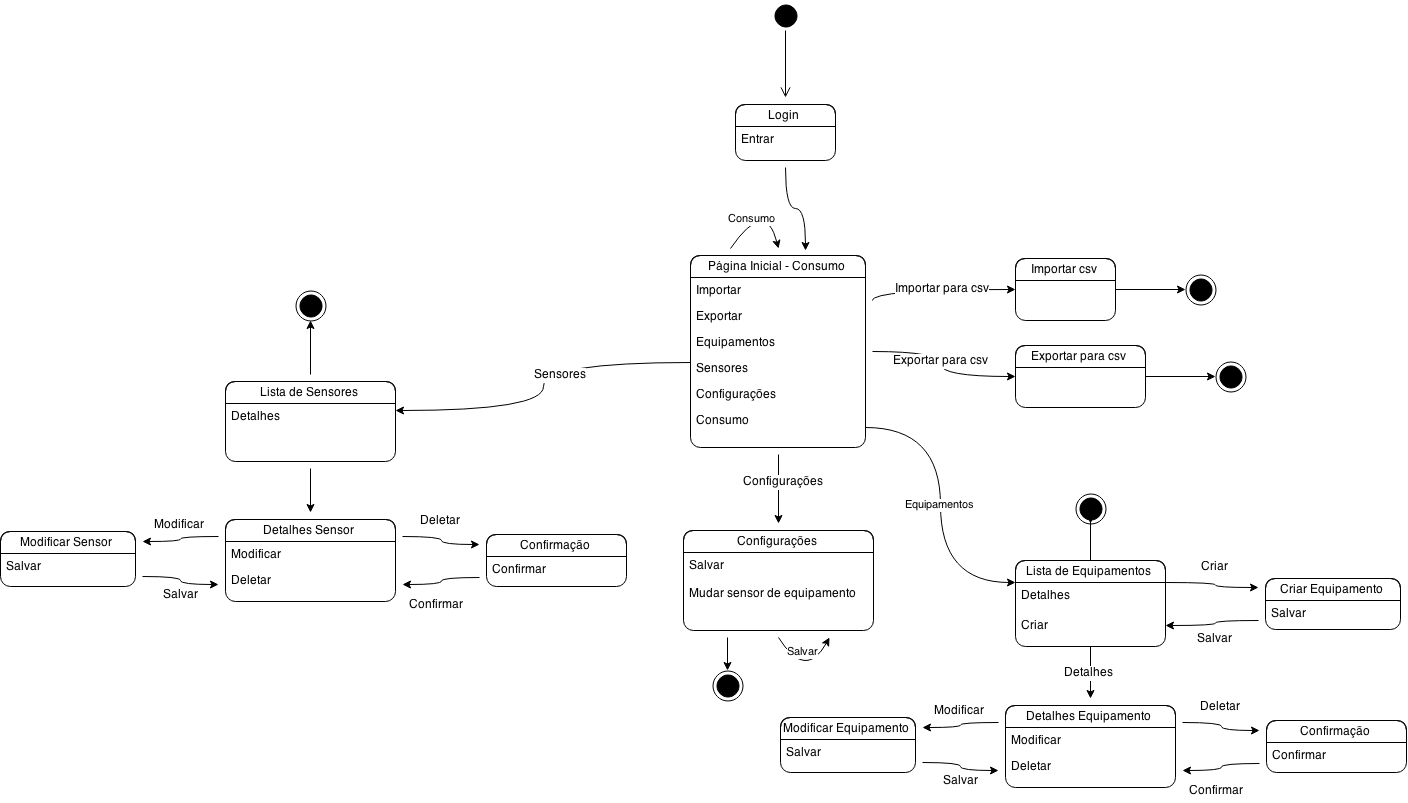
\includegraphics[width=10cm,height=10cm,keepaspectratio]{figuras/diagrama_navegacao.png}
\caption{\label{fig:diagrama navegacao} Diagrama de Navegação}
\end{center}
\end{figure}

\begin{figure}[H]
\begin{center}
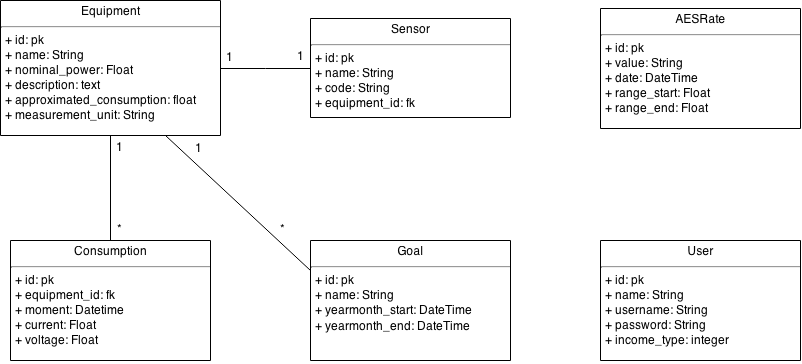
\includegraphics[width=10cm,height=10cm,keepaspectratio]{figuras/diagrama_classes.png}
\caption{\label{fig:diagrama classes} Diagrama de Classes}
\end{center}
\end{figure}

\subsection{Regras de negócio}
\paragraph{As medidas serão feitos em uma taxa de uma vez a cada dez minutos, o que leva a 6 amostras por hora, 144 por dia e 4320 por mês. Dado que cada amostra é uma linha de uma tabela, torna-se necessário algum tipo de redução desses dados para que o banco na nuvem não chegue a seu ponto máximo, dado que no projeto será usado um serviço cloud com taxa gratuita e, portanto, muito limitada. Logo, foi decidido que a janela temporal que o usuário conseguirá visualizar será restrita ao mês anterior e o mês atual quando o gráfico for uma função das horas do dia, e os outros dados mais antigos serão agrupados em meses para que ainda possa ser possível visualiza-los quando o gráfico for uma função dos meses. Caso seja necessário, será usado um plano pago, o que resolveria esse problema.
}

\subsection{Tecnologia}
\paragraph{Para o aplicativo será utilizado o framework Django, devido ao uso da linguagem python, que é uma linguagem limpa, de fácil utilização e com ampla disponibilidade de bibliotecas gratuitas e de fóruns para auxílio na implementação.
}
\mychapter{Projeto e Implementação}
\label{Cap:implementacao}
\section{Raspberry Pi}
\label{Sec:raspberry}
\subsection{Sistema Operacional}
\paragraph{
	Raspberry Pi é um computador
}
\subsection{Adaptador Wifi}
\paragraph{
	Após o sistema Raspian ser instalado no cartão de memória, foi necessário configurar o adaptador Wifi. O modelo usado é o TP-Link TL-WN723N.
}
\paragraph{
	Após o sistema Raspian ser instalado no cartão de memória, foi necessário configurar o adaptador Wifi. O modelo usado é o TP-Link TL-WN723N.
}
\begin{lstlisting}
wget https://dl.dropboxusercontent.com/u/80256631/8188eu-3.18.11-v7-781.tar.gz
tar xzf 8188eu-3.18.11-v7-781.tar.gz
./install.sh
\end{lstlisting}

\begin{table}
\centering
{\renewcommand{\arraystretch}{1.5}
\renewcommand{\tabcolsep}{0.2cm}
\begin{tabular}{|l|r|r|r|r|r|}
\hline
Componentes & qtd & Total(R\$) & Total(\$) \\
\hline
XBee 2mW PCB Antenna & 4 & {} & \$103,80 \\
XBee Explorer Dongle & 1 & {} & \$24,95 \\
Kit Raspberry Pi2 & 1 & R\$309,89 & {} \\
Sensores de Corrente & 3 & {} & \$29,85 \\
XBee Shield & 3 & {} & \$44,85 \\
Arduino Stackable Header Kit & 4 & {} & \$6,00 \\
Arduino Uno - R3 & 3 & R\$ 137,70 & {} \\
\hline
\multicolumn{2}{|l|}{Totais} & R\$447,59 & \$209,45 \\
\hline
\end{tabular}}
\caption{\label{tab:orcamento} Orçamento do projeto.}
\end{table}

\section{Some \LaTeX{} Examples}
\label{sec:examples}

\subsection{How to Leave Comments}

Comments can be added to the margins of the document using the \todo{Here's a comment in the margin!} todo command, as shown in the example on the right. You can also add inline comments:

\todo[inline, color=green!40]{This is an inline comment.}

\subsection{How to Include Figures}

First you have to upload the image file (JPEG, PNG or PDF) from your computer to writeLaTeX using the upload link the project menu. Then use the includegraphics command to include it in your document. Use the figure environment and the caption command to add a number and a caption to your figure. See the code for Figure \ref{fig:frog} in this section for an example.

\begin{figure}
\centering
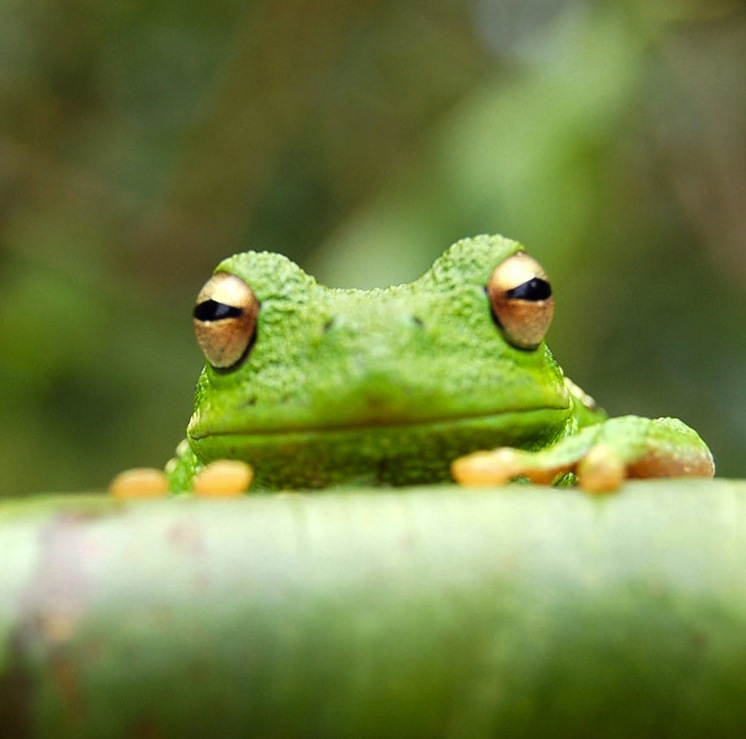
\includegraphics[width=0.3\textwidth]{frog.jpg}
\caption{\label{fig:frog}This frog was uploaded to writeLaTeX via the project menu.}
\end{figure}

\subsection{How to Make Tables}

Use the table and tabular commands for basic tables --- see Table~\ref{tab:widgets}, for example.

\begin{table}
\centering
\begin{tabular}{l|r}
Item & Quantity \\\hline
Widgets & 42 \\
Gadgets & 13
\end{tabular}
\caption{\label{tab:widgets}An example table.}
\end{table}

\subsection{How to Write Mathematics}

\LaTeX{} is great at typesetting mathematics. Let $X_1, X_2, \ldots, X_n$ be a sequence of independent and identically distributed random variables with $\text{E}[X_i] = \mu$ and $\text{Var}[X_i] = \sigma^2 < \infty$, and let
$$S_n = \frac{X_1 + X_2 + \cdots + X_n}{n}
      = \frac{1}{n}\sum_{i}^{n} X_i$$
denote their mean. Then as $n$ approaches infinity, the random variables $\sqrt{n}(S_n - \mu)$ converge in distribution to a normal $\mathcal{N}(0, \sigma^2)$.

\subsection{How to Make Sections and Subsections}

Use section and subsection commands to organize your document. \LaTeX{} handles all the formatting and numbering automatically. Use ref and label commands for cross-references.

\subsection{How to Make Lists}

You can make lists with automatic numbering \dots

\begin{enumerate}
\item Like this,
\item and like this.
\end{enumerate}
\dots or bullet points \dots
\begin{itemize}
\item Like this,
\item and like this.
\end{itemize}
\dots or with words and descriptions \dots
\begin{description}
\item[Word] Definition
\item[Concept] Explanation
\item[Idea] Text
\end{description}

We hope you find write\LaTeX\ useful, and please let us know if you have any feedback using the help menu above.

\backmatter

\bibliographystyle{apa}
\nocite{*}
\bibliography{bibliografia}

\end{document}